% !TeX spellcheck = cs_CZ
%{\tikzset{external/prefix={tikz/FYZII/}}
% \tikzset{external/figure name/.add={ch27_}{}}
%---------------------------------------------------------------------------------------------------
% file fey2ch27.tex
%---------------------------------------------------------------------------------------------------
%=========================== Kapitola Energie pole a hybnost pole ==================================
\setchaptertoc
\chapter{Energie pole a hybnost pole}\label{fyz:IIchapXXVII}
  \section{Lokální zákony zachování}\label{fyz:IIchapXXVIIsecI}
    
    Je nám jasné, že energie látky se nezachovává. Vyzařuje-li nějaký objekt světlo, ztrácí přitom
    energii. Ztracenou energii však můžeme vyjádřit v jiné formě, řekněme ve formě světelné energie.
    Proto zákon zachování energie není úplný, neuvažujeme-li i energii, která je spojená se světlem,
    přesněji s elektromagnetickým polem. Nyní se podívejme na zákon zachování energie pro pole spolu
    se zákonem zachování hybnosti. Tyto věci nemůžeme uvažovat odděleně, protože v teorii relativity
    jsou to různé stránky téhož \emph{čtyřvektoru}.
    
    Už na začátku, v prvním díle, když jsme hovořili o zákonu zachování energie, jsme si řekli, že
    celková energie na světě je konstantní. Nyní chceme myšlenku zákona zachování energie zobecnit
    takovým způsobem, abychom detailně věděli, jak se energie zachovává. Nový zákon nám bude říkat,
    že ztrácí-li se energie v dané oblasti, je to proto, že vytéká ven přes hranice této oblasti. Je
    to silnější tvrzení než prosté zachování energie bez podobných ohraničení.
    
    Abychom lépe pochopili význam našeho tvrzení, podívejme se, jak je to se zákonem zachování
    náboje. Při popisu zachování náboje jsme řekli, že existuje proudová hustota \(\vec{j}\) a
    nábojová hustota \(\varrho\), že pokles velikosti náboje v nějaké oblasti musíí být provázen
    tokem náboje ven z této oblasti. Nazývali jsme to zachování náboje. Matematická formulace zákona
    zachování je
    \begin{equation}\label{fyz:eq958}
      \nabla\cdot\vec{j}=-\diffp{\varrho}{t}.
    \end{equation}
    
    Důsledkem tohoto zákona je konstantnost celkového náboje na světě - náboj nikdy nevzniká ani
    nezaniká.
    
    Celkový náboj se však může zachovávat i jiným způsobem. Předpokládejme, že v okolí nějakého bodu
    \((1)\) je náboj \(Q_1\), zatímco v nedalekém bodě \((2)\) není žádný náboj (obr.
    \ref{fyz:fig609}). Nechť se začne náboj \(Q_1\) postupně zmenšovat a zároveň s poklesem \(Q_1\)
    se v okolí bodu \((2)\) objevuje náboj \(Q_2\) takovým způsobem, že suma \(Q_1 + Q_2\) je v
    každém okamžiku konstantní. Jinými slovy, v libovolném okamžiku množství náboje, které ubylo z
    \(Q_1\), přibude \(Q_2\). Pak bude celkové množství náboje na světě zachováno. Je to
    „celosvětové“ zachování, a ne to, čemu se říká „lokální“ zachování, protože k tomu, aby se náboj
    dostal z \((1)\) do \((2)\), se nemusel objevovat někde v prostoru mezi body \((1)\) a \((2)\).
    Lokálně se náboj prostě „ztratil“.

    \begin{figure}[ht!]   % \ref{fyz:fig609}
      \centering
      \subcaptionbox{\(Q_1+Q_2\) je konstantní\label{fyz:fig609a}}
        {\luafigure[0.8]{fyz_fig609a.pdf}}  \\
      \subcaptionbox{\(\diff{Q_1}{t} = −∫\vec{j}\cdot\vec{n}\dd{S} =
        −\diff{Q_2}{t}\)\label{fyz:fig609b}}
        {\luafigure[0.8]{fyz_fig609b.pdf}} 
      \caption{Dva způsoby zachovávání náboje. (\cite[s.~493]{Feynman02})}
      \label{fyz:fig609}
    \end{figure}

    S takovýmto „celosvětovým“ zákonem zachování jsou však v teorii relativity problémy. Pojem
    „současného okamžiku“ v navzájem vzdálených bodech není stejný pro různé soustavy. Dvě události,
    které jsou současné v jedné soustavě, nejsou současné v druhé soustavě, která se vzhledem k
    první pohybuje. V „celosvětovém“ zachování, jak jsme jej popsali, je důležité, že náboj, který
    ubyl z \(Q_1\), se \emph{zároveň} objevil v \(Q_2\). Jinak by existovaly určité okamžiky, v
    nichž by se náboj nezachovával. Zdá se, že jediný způsob, jak udělat zákon zachování
    relativisticky invariantním, je udělat z něj „lokální“ zákon zachování. Ve skutečnosti požadavek
    Lorentzovy relativistické invariantnosti překvapujícím způsobem omezuje různé zákony přírody.
    Například v moderní kvantové teorii pole se lidé často snažili pozměnit teorii zavedením
    „nelokální“ interakce, při níž něco \emph{zde} přímo ovlivnilo něco \emph{tam} - vždy však
    narazili na problémy spojené s principem relativity.

    „Lokální“ zachování je založeno na jiné myšlence. Ta říká, že náboj se může dostat z jednoho
    místa do druhého jen tehdy, kdy se stane něco v prostoru mezi těmito místy. K formulaci
    takovéhoto zákona potřebujeme nejen hustotu \(\varrho\), ale i veličinu jiného druhu, jmenovitě
    vektor \(\vec{j}\), který udává rychlost protékání náboje povrchem. Pak je vztah mezi tokem a
    časovou změnou hustoty určen rovnicí (\ref{fyz:eq957}). Je to silnější formulace zákona
    zachování. Říká, že náboj se zachovává speciálním způsobem - zachovává se „lokálně“.

    Ukazuje se, ža zachovávání energie je také \emph{lokální} proces. V dané prostorové oblasti
    definujeme kromě hustoty energie ještě i vektor, který představuje rychlost toku energie nějakým
    povrchem. Například září-li nějaký zdroj svěda, můžeme najít energii, která z něj vychází.
    Představíme-li si nějaký matematický povrch, který obklopuje světelný zdroj, energie, která se
    ztratí z tohoto ohraničeného prostoru, musí být rovna energii, která proteče příslušným
    povrchem.

  \section{Zákon zachování energie a elektromagnetizmus}\label{fyz:IIchapXXVIIsecII}
    
    Nyní bychom chtěli kvantitativně popsat zákon zachování energie v elektromagnetizmu. Abychom to
    mohli udělat, potřebujeme vědět, kolik energie obsahuje libovolný elementární objem a jaká je
    rychlost toku energie. Uvažujme nejdříve jen energii elektromagnetického pole. Nechť \(u\)
    představuje \textbf{hustotu energie pole} (tj. množství energie v jednotce objemu) a dále vektor
    \(\vec{S}\) \textbf{hustotu toku energie pole} (tj. množství energie procházející za jednotku
    času jednotkovou plochou kolmou na směr toku). Pak můžeme v úplné analogii se zákonem zachování
    náboje (viz rovnici \eqref{fyz:eq958}) psát „lokální“ zákon zachování energie pole ve tvaru
    \begin{equation}\label{fyz:eq959}
      \diff{u}{t}=-\nabla\cdot\vec{S}.
    \end{equation}
    Samozřejmě, obecně to neplatí, není pravda, že energie pole se zachovává. Představme si, že jsme
    v tmavé místnosti a náhle rozsvítíme svědo. V okamžiku je místnost plná světla, tj. objevila se
    energie pole, která tu předtím nebyla. Rovnice \eqref{fyz:eq959} nepředstavuje úplný zákon
    zachování, neboť se nezachovává energie samotného pole, ale jen celková energie na světě, neboť
    je tu také energie látky. Energie pole se změní, vykonává-li se práce působením látky na pole
    nebo opačně.
    
    Je-li však v objemu, který nás zajímá, nějaká látka, víme, kolik energie představuje: každá
    částice má energii \(m_0c^2/\sqrt{1-v^2/c^2}\). Celková energie látky je součtem energií všech
    částic a tok této energie povrchem je součtem energií částic, které povrchem procházejí. Nyní
    chceme hovořit jen o energii elektromagnetického pole. Proto hledáme rovnice, které říkají, že
    celková energie pole v daném objemu se zmenšuje \emph{buď} proto, že energie teče ven z objemu,
    \emph{nebo} proto, že pole odevzdává energii látce (nebo ji od něj získává, což je vlastně
    záporná ztráta). Energie pole uvnitř objemu \(V\) je
    \begin{equation*}
      \int_Vu\dd{V},
    \end{equation*}
    a rychlost jejího poklesu je rovna časové derivaci tohoto integrálu se záporným znaménkem. Tok
    energie z objemu \(V\) je roven integrálu kolmé složky \(\vec{S}\) povrchem \(S\), který
    ohraničuje objem \(V\):
    \begin{equation*}
      \int_\Sigma\vec{S}\cdot\vec{n}\dd{S}.
    \end{equation*}
    Proto
    \begin{equation}\label{fyz:eq960}
      \begin{multlined}
        -\diff{}{t}\int_Vu\dd{V}=\int_\Sigma\vec{S}\cdot\vec{n}\dd{S} + \\
        + (\text{práce vykonaná na látce uvnitř \(V\)}).
      \end{multlined}
    \end{equation}

  \section{Hustota energie a hustota toku energie elektromagnetického 
    pole}\label{fyz:IIchapXXVIIsecIII}
  \section{Nejednoznačnost energie pole}\label{fyz:IIchapXXVIIsecIV}
  \section{Příklady hustoty toku energie}\label{fyz:IIchapXXVIIsecV}
  \section{Hybnost pole}\label{fyz:IIchapXXVIIsecVI}
    \begin{equation}\label{fyz:eq957}
      \vec{g}=\frac{1}{c^2}\,\vec{S}.
    \end{equation}
  \section{Příklady a cvičení}\label{fyz:IIchapXXVIIsecVII}





    \begin{figure}[ht!] %\ref{fyz:fig610}
      \centering
      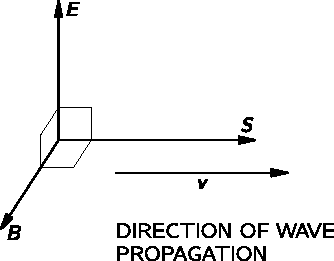
\includegraphics[width=0.7\linewidth]{fyz_fig610.pdf}
      \caption{
               (\cite[s.~707]{Feynman02})}
      \label{fyz:fig610}
    \end{figure}

    \begin{figure}[ht!] %\ref{fyz:fig611}
      \centering
      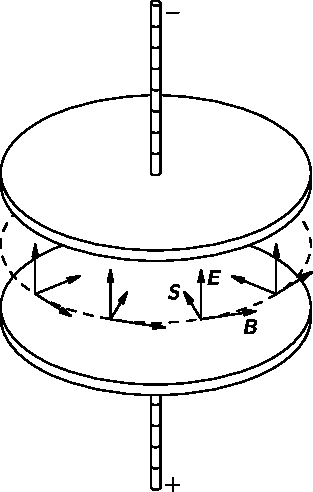
\includegraphics[width=0.7\linewidth]{fyz_fig611.pdf}
      \caption{
               (\cite[s.~707]{Feynman02})}
      \label{fyz:fig611}
    \end{figure}

    \begin{figure}[ht!] %\ref{fyz:fig612}
      \centering
      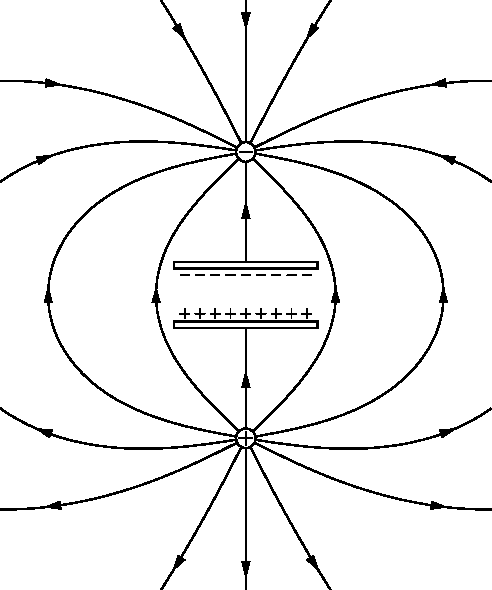
\includegraphics[width=0.7\linewidth]{fyz_fig612.pdf}
      \caption{
               (\cite[s.~707]{Feynman02})}
      \label{fyz:fig612}
    \end{figure}

    \begin{figure}[ht!] %\ref{fyz:fig613}
      \centering
      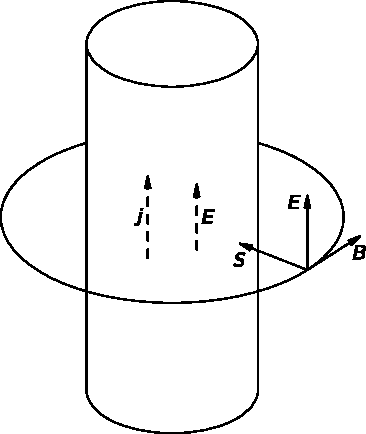
\includegraphics[width=0.7\linewidth]{fyz_fig613.pdf}
      \caption{
               (\cite[s.~707]{Feynman02})}
      \label{fyz:fig613}
    \end{figure}

    \begin{figure}[ht!] %\ref{fyz:fig614}
      \centering
      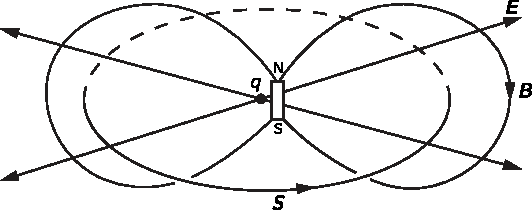
\includegraphics[width=0.7\linewidth]{fyz_fig614.pdf}
      \caption{
               (\cite[s.~707]{Feynman02})}
      \label{fyz:fig614}
    \end{figure}

    \begin{figure}[ht!] %\ref{fyz:fig615}
      \centering
      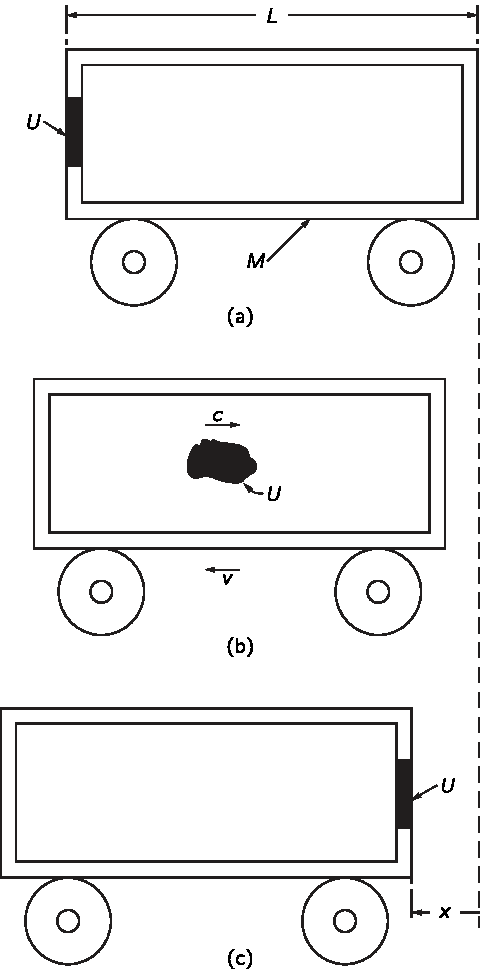
\includegraphics[width=0.7\linewidth]{fyz_fig615.pdf}
      \caption{
               (\cite[s.~707]{Feynman02})}
      \label{fyz:fig615}
    \end{figure}

    \begin{figure}[ht!] %\ref{fyz:fig616}
      \centering
      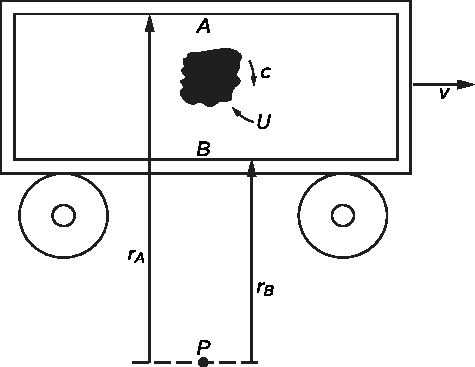
\includegraphics[width=0.7\linewidth]{fyz_fig616.pdf}
      \caption{
               (\cite[s.~707]{Feynman02})}
      \label{fyz:fig616}
    \end{figure}

    \todo[inline]{Kapitola fey2ch27 je nedodělaná, obsahuje pouze obrázky}
%} %tikzset
%---------------------------------------------------------------------------------------------------